\documentclass[11pt]{article}
\usepackage[margin=1in]{geometry}
\usepackage[T1]{fontenc}
\usepackage{amsmath,amssymb}
\usepackage{graphicx}
\usepackage{booktabs}
\usepackage{caption}
\usepackage{microtype}
\usepackage{cite}
\usepackage[colorlinks=true,linkcolor=blue,citecolor=blue,urlcolor=blue]{hyperref}

\graphicspath{{figures/}}
\captionsetup{font=small,labelfont=bf}
\newcommand{\mc}{m_c}
\newcommand{\code}[1]{\texttt{#1}}
\newcommand{\cT}{\mathcal{T}}
\newcommand{\cU}{\mathcal{U}}
\newcommand{\nrm}[2]{\lVert #1\rVert_{#2}}
\newcommand{\Dm}{\Delta m}

\title{Why does rewording flip a refusal?\\A perturbation analysis of Gemma-2-2b-it}
\author{[author]}
\date{Draft of 23 November 2026}

\begin{document}
\maketitle

\begin{abstract}
A small change in the wording of a request can flip a chat model between refusing and answering. We ask whether this happens because the model amplifies the change as it passes through the layers, and whether the flip can be predicted from a linearized description of the model. For Gemma-2-2b-it the answer to the first question is no. The difference between two wordings shrinks in relative size with depth, to 0.42 of its starting value when measured over all tokens. Random perturbations shrink in the same way, whether they are made at one token or at every token of the user's text. A narrow set of directions close to the gradient of the output is amplified about 10 to 40 times, but a real rewording has a component of at most 1\% along them. The answer to the second question is mixed. Once the two wordings are known, the gradient times the difference in internal state predicts the change in the output with correlation 0.92 and slope 0.99. From the original prompt alone, three predictors of how often rewording flips it do no better than the prompt's distance from the refusal threshold. The gradient is largely one direction shared by all prompts; on real prompts it reads the same coordinate as the known refusal direction (correlation 0.96), although the two vectors have a cosine of only 0.2 to 0.3. The picture that fits the measurements is the one known from adversarial examples, a damped system with one steep direction: a rewording flips a prompt when the prompt is near the threshold and the rewording's small component along the steep direction is enough to cross it. The difference between two wordings is written into the positions that decide the output at layers 7, 11 and 13, mostly by about ten attention heads that are largely the same across prompts; this last statement is an attribution and has not been tested by intervention.
\end{abstract}

\section{Question and approach}
\label{sec:question}

The starting point is an analogy with perturbation theory. A transformer applies 26 layers in sequence to a set of state vectors, one per token. Two wordings of the same request give two initial states that differ slightly. If the layers amplified such differences, small changes of wording would have large effects, and the most amplified directions would say which changes matter.

This suggests two measurements and one test.

\begin{description}
\item[Amplification.] Add a perturbation to the state at some layer, follow it to the last layer, and compare its relative size at the end with its relative size at the start. Do the same for the difference between two real wordings (Section~\ref{sec:gain}).
\item[Linear response.] Compute the gradient of the output with respect to the state, and check whether the gradient times the difference in state between two wordings gives the change in the output (Section~\ref{sec:linresp}).
\item[The test.] Predict, from one prompt alone, how likely a rewording is to flip its outcome, using the gradient and the statistics of the displacements that rewordings cause in other prompts (Section~\ref{sec:testdef}). The test was fixed in advance to count only if this beats the prompt's distance from the refusal threshold alone.
\end{description}

A feature-level version of the same description, in terms of interpretable dictionary features, was planned and could not be carried out (Section~\ref{sec:features}).

Much of the picture that results is known in other settings. Section~\ref{sec:related} says which parts are published and which measurements appear to be new.

\section{Definitions and methods}
\label{sec:setup}

This section defines every quantity used in the results. Readers who want the findings first can go to Section~\ref{sec:results} and return here for the definitions.

\subsection{Model, positions and notation}
\label{sec:notation}

The model is \code{google/gemma-2-2b-it}, the 2-billion-parameter chat model. All runs are in 32-bit floating point on one laptop.

A prompt $x$ is turned into a sequence of $T$ tokens. The model keeps one state vector per token and updates it in 26 layers. We write
\begin{equation}
h_\ell(t)\in\mathbb{R}^d,\qquad d=2304,\qquad t=1,\dots,T,\qquad \ell=-1,0,1,\dots,25,
\end{equation}
for the state at token position $t$ after layer $\ell$, with $\ell=-1$ for the token embeddings before any layer. Each layer adds to the state, $h_\ell=h_{\ell-1}+F_\ell(h_{\ell-1})$. The update $F_\ell$ has two parts. \emph{Attention} moves information between positions, and only forwards: the state at position $t$ can read from positions $t'\le t$. It is carried out by 8 parallel \emph{attention heads} per layer, 208 in all. The second part acts on each position separately. The probabilities of the first output token are computed from the single vector $h_{25}(T)$.

Each prompt is one user turn in the model's chat template, with no system prompt. Its tokens fall into three groups:
\begin{itemize}
\item four fixed tokens that open the turn, identical in every prompt and never perturbed;
\item the user's text, at positions we call $\cU$ (a median of 14 tokens);
\item five fixed tokens that close the turn and open the model's reply, the \emph{template positions} $\cT$.
\end{itemize}
We write $S=\cU\cup\cT$. Because the template tokens are the same in every prompt, the five positions in $\cT$ are the only ones that can be compared between prompts of different length.

For a set of positions $P$ and a quantity $v$ with one vector per position, the norm over $P$ is
\begin{equation}
\nrm{v}{P}=\Bigl(\sum_{t\in P}\lVert v(t)\rVert^2\Bigr)^{1/2},
\label{eq:norm}
\end{equation}
the Euclidean norm of the vectors at those positions stacked into one long vector. A dot product over $P$ is defined in the same way, $a\cdot b=\sum_{t\in P}a(t)\cdot b(t)$.

\subsection{The output scalar and the outcome}
\label{sec:mdef}

Let $p_{\rm I}(x)$ be the probability the model assigns to ``I'' as its first output token, as in ``I cannot''. The output scalar is its log-odds,
\begin{equation}
m(x)=\ln\frac{p_{\rm I}(x)}{1-p_{\rm I}(x)} .
\label{eq:m}
\end{equation}
So $m=0$ means $p_{\rm I}=1/2$, and one unit of $m$ multiplies the odds by $e$.

The \emph{outcome} is what the model writes. A completion of at most 48 tokens is generated greedily (always taking the most probable token) and labelled refused, answered or unclear by a rule-based judge. $m$ is a proxy for this label, and three numbers describe how good a proxy it is.
\begin{itemize}
\item The \emph{ranking probability} (the area under the ROC curve): the probability that a randomly chosen refused prompt has a larger $m$ than a randomly chosen answered one. It is 1 for a perfect proxy and $1/2$ for a useless one.
\item The \emph{threshold} $\mc$: the value of $m$ that best separates the two labels. It maximizes the average of two fractions, the refused prompts with $m>\mc$ and the answered prompts with $m\le\mc$. The result is $\mc=-0.23$, which corresponds to $p_{\rm I}=0.44$.
\item The \emph{width} $s$ of the transition, from a logistic curve fitted by maximum likelihood to the labels of 1{,}085 prompts,
\begin{equation}
\Pr(\text{refused}\mid m)=\frac{1}{1+\exp[-(m-m_0)/s]},\qquad m_0=-0.42,\quad s=0.80 .
\label{eq:logistic}
\end{equation}
The fitted fraction refused rises from 27\% to 73\% as $m$ goes from $m_0-s$ to $m_0+s$.
\end{itemize}
The curve~(\ref{eq:logistic}) is used only to calibrate $m$ against the judged label. It plays no part in the flip test of Section~\ref{sec:testdef}, where a flip is defined on $m$ itself.

\subsection{Prompts, rewordings and flips}
\label{sec:prompts}

A pool of 5{,}311 prompts was built from six public benchmarks: AdvBench \cite{advbench}, HarmBench \cite{harmbench}, JailbreakBench \cite{jbb}, OR-Bench \cite{orbench}, XSTest \cite{xstest} and Alpaca \cite{alpaca}. From it, 120 prompts were chosen to cover eight ranges of the signed distance $m-\mc$, 15 in each, four on the answering side ($m<\mc$) and four on the refusing side.

Each of the 120 prompts has 20 rewordings of four kinds (Table~\ref{tab:kinds}). This gives 2{,}520 prompts and 2{,}400 \emph{pairs} $(x,x')$ of an original and a rewording. For a pair we write
\begin{equation}
\Dm=m(x')-m(x),
\end{equation}
and the pair is a \emph{flip} when the two values lie on opposite sides of the threshold,
\begin{equation}
y=\begin{cases}1 & \text{if } \bigl(m(x')-\mc\bigr)\bigl(m(x)-\mc\bigr)<0,\\ 0 & \text{otherwise.}\end{cases}
\label{eq:flip}
\end{equation}
The flip is defined on $m$ and not on the judged label, because near the threshold about one completion in six has no clear label.

\begin{table}[ht]
\centering
\caption{The four kinds of rewording. T0 uses the same five recipes for every prompt. T1 to T3 were written by a language model and checked automatically.}
\label{tab:kinds}
\begin{tabular}{llcl}
\toprule
Kind & What changes & Per prompt & Written by \\
\midrule
T0 & punctuation, capitalization or spacing & 5 & code \\
T1 & one or two words & 5 & language model \\
T2 & full rephrasing with the same meaning & 6 & language model \\
T3 & register, or one added clause of context & 4 & language model \\
\bottomrule
\end{tabular}
\end{table}

\subsection{Size of a perturbation and relative gain}
\label{sec:gain}

\paragraph{Relative size.} Let $\delta$ be a perturbation of the state at layer $\ell$, or the difference between the states of two prompts there. Its size is always quoted relative to the state it belongs to, over a stated set of positions $P$:
\begin{equation}
\varepsilon_\ell(\delta;P)=\frac{\nrm{\delta}{P}}{\nrm{h_\ell}{P}} .
\label{eq:eps}
\end{equation}

\paragraph{Following a perturbation.} Replace $h_\ell$ by $h_\ell+\delta$, run the remaining layers, and let $\delta'$ be the resulting change of the state at a later layer $\ell'$. The \emph{relative gain} is
\begin{equation}
R(\ell\to\ell')=\frac{\varepsilon_{\ell'}(\delta';P')}{\varepsilon_\ell(\delta;P)} .
\label{eq:gain}
\end{equation}
$R>1$ means the perturbation has grown relative to the state and $R<1$ that it has shrunk. The norm of the state itself grows about 12.6 times from the embeddings to the last layer; dividing by it in~(\ref{eq:eps}) keeps that growth from being counted as amplification. Three choices of positions are used.
\begin{itemize}
\item \emph{One token:} the perturbation is made at one position $t$ and both sizes are taken at that position, $P=P'=\{t\}$. Then $R=1$ at $\ell'=\ell$.
\item \emph{All tokens:} the perturbation is made at the positions of the user's text and both sizes are taken over $S$, $P=P'=S$. Again $R=1$ at $\ell'=\ell$.
\item \emph{Template:} the same perturbation, with the change measured at the template positions only, $P=S$ and $P'=\cT$. This starts at 0, because nothing has yet reached the template positions, and measures how strongly the positions that decide the output are disturbed.
\end{itemize}

\paragraph{Finite and linearized.} The \emph{finite} gain comes from actually rerunning the model with $h_\ell+\delta$. The \emph{linearized} gain is the limit of an infinitesimal perturbation, $\delta'=J\,\delta$, where $J=\partial h_{\ell'}/\partial h_\ell$ is the Jacobian of the layers in between. The product $J\delta$ is computed exactly by forward-mode differentiation, without forming $J$. The two agree to a few percent at $\varepsilon\le 0.03$ for every direction except the gradient (Section~\ref{sec:amplified}).

\paragraph{Deviation from linearity.} For a perturbation of size $\varepsilon$ along a fixed direction, made with both signs, the changes $\delta'(+\varepsilon)$ and $\delta'(-\varepsilon)$ of a later state separate into a part that is odd in $\varepsilon$ and a part that is even,
\begin{equation}
\delta'_{\rm odd}=\tfrac12\bigl[\delta'(+\varepsilon)-\delta'(-\varepsilon)\bigr],\qquad
\delta'_{\rm even}=\tfrac12\bigl[\delta'(+\varepsilon)+\delta'(-\varepsilon)\bigr].
\label{eq:oddeven}
\end{equation}
The linear response is in the odd part and the leading nonlinear (second-order) term is the even part. With $D=\delta'_{\rm odd}(\varepsilon_0)/\varepsilon_0$ the linear response per unit size, taken at the smallest size $\varepsilon_0=0.01$, the deviation from linearity at size $\varepsilon$ is
\begin{equation}
\nu(\varepsilon)=\frac{\lVert\delta'(\varepsilon)-\varepsilon D\rVert}{\lVert\varepsilon D\rVert},
\label{eq:nu}
\end{equation}
and $\nu_m$ is the same quantity for the scalar $m$. Where second order dominates, $\nu\simeq\kappa\,\varepsilon$, and we quote $\kappa=\lVert\delta'_{\rm even}\rVert/(\varepsilon\,\lVert\delta'_{\rm odd}\rVert)$ at $\varepsilon=0.03$. The \emph{linear range} is the size at which $\nu$ reaches 0.3. To say how far a perturbation $\delta$ leaves the cloud of real states we use its Mahalanobis length $\sqrt{\delta^{\mathsf T}C^{-1}\delta/d}$, with $C$ the covariance of the states of the 5{,}311 pool prompts at that layer and position; a difference between two real states has a length of order 1 to 2 in these units.

\paragraph{Directions.} With $u$ a unit vector in $\mathbb{R}^d$ and $c$ a constant that sets the total size $\varepsilon$:
\begin{itemize}
\item \emph{isotropic random:} $u=z/\lVert z\rVert$ with $z$ a standard Gaussian vector;
\item \emph{covariance-matched random:} $u\propto(1-\hat r\hat r^{\mathsf T})\,C^{1/2}z$, where $C$ is the covariance of the states of different prompts at that layer and $\hat r$ is the refusal direction of Section~\ref{sec:scalar}, projected out so that the baseline does not contain it;
\item \emph{one token:} $\delta(t)=c\,u$ at a single position;
\item \emph{same direction at every token:} $\delta(t)=c\,\lVert h_\ell(t)\rVert\,u$ for all $t\in\cU$;
\item \emph{independent at every token:} $\delta(t)=c\,\lVert h_\ell(t)\rVert\,u_t$ with a separate draw $u_t$ for each $t\in\cU$;
\item \emph{gradient:} $\delta(t)=c\,g_\ell(t)$, with $g_\ell$ defined in Section~\ref{sec:linresp};
\item \emph{real rewording:} $\delta(t)=c\,\Delta_\ell(t)$, the measured difference between two wordings, defined next.
\end{itemize}

\paragraph{Real rewordings.} For a pair $(x,x')$ the displacement at layer $\ell$ is
\begin{equation}
\Delta_\ell(t)=h^{x'}_\ell(t)-h^{x}_\ell(t) .
\label{eq:Delta}
\end{equation}
At the template positions this is defined for every pair. At the positions of the user's text it needs a one-to-one match between the tokens of the two prompts, which exists when the edit replaces $k$ tokens by $k$ tokens; this holds for 543 of the 1{,}200 pairs of kinds T0 and T1. For those pairs we follow $\varepsilon_\ell(\Delta_\ell;S)$ through the layers and report it divided by its value at the embeddings, $\varepsilon_\ell/\varepsilon_{-1}$. No perturbation is injected here: the two prompts are simply run, so a ratio above 1 would be amplification by the model.

\paragraph{Effective number of tokens.} How many positions a difference is spread over is measured by the participation ratio
\begin{equation}
N_{\rm eff}=\frac{\bigl(\sum_t w_t\bigr)^2}{\sum_t w_t^2},\qquad w_t=\lVert\delta(t)\rVert^2 ,
\label{eq:neff}
\end{equation}
which is 1 when the difference sits at one position and $N$ when it is spread equally over $N$.

\subsection{Gradient and linear response}
\label{sec:linresp}

The gradient of the output scalar with respect to the state at layer $\ell$ and position $t$ is
\begin{equation}
g_\ell(t)=\frac{\partial m}{\partial h_\ell(t)}\in\mathbb{R}^d ,
\label{eq:g}
\end{equation}
where the state at layer $\ell$ is treated as the independent variable and all later layers are differentiated through. It is computed by reverse-mode differentiation for the original prompt $x$.

\paragraph{Linear prediction.} Given the state at all positions at layer $\ell$, the output is fixed, so to first order in the displacement~(\ref{eq:Delta}),
\begin{equation}
\Dm\simeq \sum_{t\in P} g_\ell(t)\cdot\Delta_\ell(t)\equiv L_\ell .
\label{eq:lin}
\end{equation}
Summed over all positions this is the first-order Taylor expansion. We mostly use the sum over the template positions only, $P=\cT$, because it is defined for every pair. That version leaves out whatever the layers after $\ell$ still read from the user's text, so it can only be complete once the effect of the rewording has reached the template positions (Section~\ref{sec:swap}).

The quality of~(\ref{eq:lin}) over a set of pairs is described by three numbers: the Pearson correlation between $L_\ell$ and $\Dm$; the slope $b=\sum L_\ell\,\Dm/\sum L_\ell^2$ of the least-squares line through the origin, which is 1 if the prediction has the right size; and the fraction of pairs for which $L_\ell$ and $\Dm$ have the same sign, counted over the pairs with $|\Dm|>0.5$.

\paragraph{Steepness and alignment.} By the Cauchy--Schwarz inequality, among all perturbations of relative size $\varepsilon$ over $S$ the one along the gradient changes $m$ the most, by $\varepsilon\,G_\ell$ to first order, with
\begin{equation}
G_\ell=\nrm{g_\ell}{S}\,\nrm{h_\ell}{S} .
\label{eq:G}
\end{equation}
We call $G_\ell$ the \emph{steepness}: the change in $m$ per unit of relative perturbation in the most effective direction. For any other displacement the first-order change is smaller by the cosine of its angle to the gradient,
\begin{equation}
\Dm\simeq G_\ell\;\varepsilon_\ell(\Delta_\ell;S)\;\cos\theta_\ell,\qquad
\cos\theta_\ell=\frac{\sum_{t\in S}g_\ell(t)\cdot\Delta_\ell(t)}{\nrm{g_\ell}{S}\,\nrm{\Delta_\ell}{S}} .
\label{eq:consistency}
\end{equation}
Equation~(\ref{eq:consistency}) separates the three things that decide the effect of a rewording: how steep the output is, how large the rewording is, and how well it is aligned with the steep direction.

\subsection{The swap experiment}
\label{sec:swap}

The template tokens are identical in the two prompts of a pair, so at the embeddings $\Delta_{-1}(t)=0$ for $t\in\cT$. The rewording can affect the output only by being read out of the user's text into the template positions by attention. The swap experiment measures by which layer this has happened.

For a pair $(x,x')$ and a layer $\ell$: run the original prompt $x$ up to layer $\ell$, replace its state at the five template positions by that of the rewording, $h^{x}_\ell(t)\to h^{x'}_\ell(t)$ for $t\in\cT$, leave the user's text as it is, and run the remaining layers. Call the resulting output $m^{\rm swap}_\ell$. Then
\begin{equation}
A_\ell=m^{\rm swap}_\ell-m(x),\qquad f_\ell=\frac{A_\ell}{\Dm} .
\label{eq:arrival}
\end{equation}
After the swap the template positions hold everything the rewording had delivered to them up to layer $\ell$, while everything read after layer $\ell$ comes from the original's text. So $f_\ell$ is the fraction of the eventual change that has \emph{arrived} at the template positions by layer $\ell$. It is 0 at the embeddings and exactly 1 at $\ell=25$. We report the median of $f_\ell$ over the pairs with $|\Dm|>0.5$, since the ratio is meaningless when $\Dm$ is near zero.

\paragraph{What each layer writes.} The increments
\begin{equation}
S_\ell=A_\ell-A_{\ell-1},\qquad \sum_{\ell=0}^{25}S_\ell=\Dm ,
\label{eq:source}
\end{equation}
split the change of $m$ exactly by the layer at which it is read into the template positions. The share of layer $\ell$ over a set of pairs $p$ is the regression weight
\begin{equation}
w_\ell=\frac{\sum_p S_\ell^{(p)}\,\Dm^{(p)}}{\sum_p \bigl(\Dm^{(p)}\bigr)^2},\qquad \sum_\ell w_\ell=1 .
\label{eq:share}
\end{equation}

\paragraph{Split by attention head.} Within layer $\ell$ the attention update at the template positions is a sum over the 8 heads. Let $u_{\ell,h}(t)$ be the change in head $h$'s contribution when it reads the rewording's text instead of the original's, with the same input at the template positions. Its first-order effect on the output is
\begin{equation}
e_{\ell,h}=\sum_{t\in\cT} g^{\rm mid}_\ell(t)\cdot u_{\ell,h}(t),
\label{eq:head}
\end{equation}
where $g^{\rm mid}_\ell$ is the gradient of $m$ with respect to the state just after the attention update of layer $\ell$. The share of a head is defined as in~(\ref{eq:share}) with $e_{\ell,h}$ in place of $S_\ell$. Unlike~(\ref{eq:source}) this split is first order, and the head shares need not add up to 1; what they add up to measures how much of the change the split accounts for. Each head's contribution is further divided by the position it reads from.

\subsection{The flip-probability test}
\label{sec:testdef}

\paragraph{The model.} Fix an original prompt with output $m$ and gradient $g$, and suppose a rewording displaces the state at the template positions at layer $\ell$ by a random $\Delta$. By~(\ref{eq:lin}) the output shifts by $\Dm=g\cdot\Delta$. If $\Delta$ has zero mean and second-moment matrix $\Sigma=\langle\Delta\Delta^{\mathsf T}\rangle$, then $\Dm$ has zero mean and variance
\begin{equation}
\sigma^2=\langle (g\cdot\Delta)^2\rangle = g^{\mathsf T}\,\Sigma\, g .
\label{eq:sigma}
\end{equation}
Here $g$ and $\Delta$ are the vectors at the five template positions stacked, of dimension $5d=11{,}520$. A flip~(\ref{eq:flip}) occurs when the shift carries $m$ across $\mc$, that is, when $\Dm$ exceeds the distance $|m-\mc|$ in the direction of the threshold. If $\Dm$ is Gaussian, the probability of that is the one-sided tail
\begin{equation}
P_{\rm flip}=\Phi\!\left(-\frac{|m-\mc|}{\sigma}\right),\qquad
\Phi(x)=\frac{1}{\sqrt{2\pi}}\int_{-\infty}^{x}e^{-t^2/2}\,dt .
\label{eq:pflip}
\end{equation}
The argument is the distance to the threshold in units of a typical shift. $P_{\rm flip}=1/2$ for a prompt at the threshold and falls to 0.16, 0.023 and 0.0013 at one, two and three $\sigma$. This is the same form as the Press--Schechter collapse fraction, with $|m-\mc|$ in place of the critical overdensity.

\paragraph{The four predictors.} All four use~(\ref{eq:pflip}); they differ only in $\sigma$. Let $f$ label the original prompt, $k$ the kind of rewording, and let the average $\langle\cdot\rangle_{k,\neg f}$ run over all pairs of kind $k$ belonging to the \emph{other} 119 prompts, and $\langle\cdot\rangle_{k,f}$ over the 4 to 6 pairs of kind $k$ of prompt $f$ itself.
\begin{align}
\text{distance to the threshold:}\quad & \sigma^2_{f,k}=\bigl\langle \Dm^2\bigr\rangle_{k,\neg f}, \label{eq:sigdist}\\
\text{gradient-based prediction:}\quad & \sigma^2_{f,k}=\bigl\langle (g_f\cdot\Delta)^2\bigr\rangle_{k,\neg f}=g_f^{\mathsf T}\,\Sigma_{k,\neg f}\,g_f, \label{eq:siggrad}\\
\text{same formula, own rewordings:}\quad & \sigma^2_{f,k}=\bigl\langle (g_f\cdot\Delta)^2\bigr\rangle_{k,f}, \label{eq:sigownlin}\\
\text{own spread:}\quad & \sigma^2_{f,k}=\bigl\langle \Dm^2\bigr\rangle_{k,f}. \label{eq:sigown}
\end{align}
In~(\ref{eq:sigdist}) every prompt gets the same $\sigma$ for a given kind of rewording, so the only thing that distinguishes one prompt from another is its distance $|m-\mc|$. This is the baseline. In~(\ref{eq:siggrad}), the prediction under test, the prompt's own gradient $g_f$ is combined with the displacements observed for other prompts; $\sigma$ is computed as the root mean square of the projections $g_f\cdot\Delta$, which equals $g_f^{\mathsf T}\Sigma g_f$ without forming the matrix. Neither~(\ref{eq:sigdist}) nor~(\ref{eq:siggrad}) uses any rewording of prompt $f$, and neither has a fitted parameter. The last two use the prompt's own rewordings and are not predictions. Equation~(\ref{eq:sigownlin}) shows how well the formula does when it is given the right displacements, and~(\ref{eq:sigown}) how well it does when it is given the prompt's true spread; the latter is the ceiling for a predictor of this form. Probabilities are clipped to the range 0.01 to 0.99.

\paragraph{The Brier score.} A set of predicted probabilities $P_i$ is scored against the outcomes $y_i\in\{0,1\}$ by the mean squared error
\begin{equation}
B=\frac{1}{N}\sum_{i=1}^{N}\bigl(P_i-y_i\bigr)^2 ,
\label{eq:brier}
\end{equation}
with $i$ running over the $N=2{,}400$ pairs and $y_i$ the flip indicator~(\ref{eq:flip}). Lower is better. $B=0$ for a perfect forecast and $B=0.25$ for always saying $1/2$. Predicting the overall flip rate $r$ for every pair gives $B=r(1-r)$, the score of a forecast with no skill; here $r=358/2400=0.149$ and $r(1-r)=0.127$. The score rewards both ranking the pairs correctly and getting the probabilities themselves right, which is why it suits a prediction with no fitted parameter.

\paragraph{Uncertainty.} Two predictors $a$ and $b$ are compared by the difference $B_a-B_b$. Its 95\% interval comes from a bootstrap over prompts: the 120 prompts are resampled with replacement 2{,}000 times, each prompt bringing all 20 of its pairs, and the interval runs from the 2.5th to the 97.5th percentile of the resampled differences. Prompts and not pairs are resampled because the pairs of one prompt share its distance from the threshold and are not independent.

\paragraph{Rank correlation.} As a second measure that looks only at the ordering, we give the Spearman rank correlation, over the 120 prompts, between the mean predicted flip probability of a prompt and the fraction of its 20 rewordings that flip.

\paragraph{Gap closed.} The room for improvement is the difference between the baseline and the ceiling. A predictor with score $B$ closes the fraction $(B_{\rm dist}-B)/(B_{\rm dist}-B_{\rm own})$ of it.

\paragraph{The assumptions.} The derivation of~(\ref{eq:pflip}) assumes linear response, zero-mean Gaussian shifts, and displacement statistics that are the same for every prompt. Linear response is tested directly (Section~\ref{sec:linear}). On the second, the measured shifts are not centred for the larger rewordings (Table~\ref{tab:tiers}), and pooled over prompts their distribution has heavier tails than a Gaussian: the excess kurtosis of $\Dm$ is 10, 11, 1.0 and 5.2 for the four kinds, against 0 for a Gaussian. Heavy tails in the pooled distribution are what one expects if each prompt has its own width. That is the third assumption, and it is the one the test shows to fail (Section~\ref{sec:test}).

\subsection{The most amplified directions}
\label{sec:svd}

For a set of source positions $P$ at layer $\ell$, let $J=\partial h_{25}(\cT)/\partial h_\ell(P)$ be the Jacobian from the state at those positions to the state at the template positions at the last layer. Its largest singular value,
\begin{equation}
\sigma_1(J)=\max_{v\ne 0}\frac{\lVert Jv\rVert}{\lVert v\rVert},
\end{equation}
is the largest factor by which any infinitesimal perturbation at $P$ is stretched, and the maximizing $v$ is the most amplified direction. Both are found by iterating products with $J$ and $J^{\mathsf T}$, without forming $J$. In relative terms, as in the template version of~(\ref{eq:gain}), the amplification is
\begin{equation}
\mathcal{A}=\sigma_1(J)\,\frac{\nrm{h_\ell}{S}}{\nrm{h_{25}}{\cT}} .
\label{eq:amp}
\end{equation}

\paragraph{A bound on collective modes.} The following is elementary linear algebra, stated to fix what ``more unstable'' can mean for a perturbation over many tokens. A perturbation over $N$ positions is a set of one-token perturbations $v(t)$, and the map is linear, $Jv=\sum_t J_t\,v(t)$, with $J_t$ the Jacobian from position $t$ alone. Therefore
\begin{equation}
\lVert Jv\rVert\le\sum_t\sigma_1(J_t)\,\lVert v(t)\rVert\le\Bigl(\sum_t\sigma_1(J_t)^2\Bigr)^{1/2}\lVert v\rVert
\quad\Longrightarrow\quad
\sigma_1(J)\le\sqrt{N}\,\max_t\sigma_1(J_t) .
\label{eq:bound}
\end{equation}
At equal total size, a perturbation spread over $N$ tokens can be amplified at most $\sqrt N$ times more than the best one-token perturbation, and it reaches that only if all $N$ tokens are equally sensitive and their effects add in the same output direction.

\subsection{Tools}

The model can be restarted from the state at any layer and gives identical output. Forward-mode and reverse-mode derivatives agree to about 2 parts in $10^5$.

\section{Results}
\label{sec:results}

\subsection{The scalar tracks the outcome, and one direction controls it}
\label{sec:scalar}

On a random sample of 600 pool prompts, the ranking probability of $m$ (Section~\ref{sec:mdef}) is 0.994. The fraction refused rises from 0.13 to 0.90 as $m$ goes from $-2$ to $+1$ (Figure~\ref{fig:reliability}).

\begin{figure}[ht]
\centering
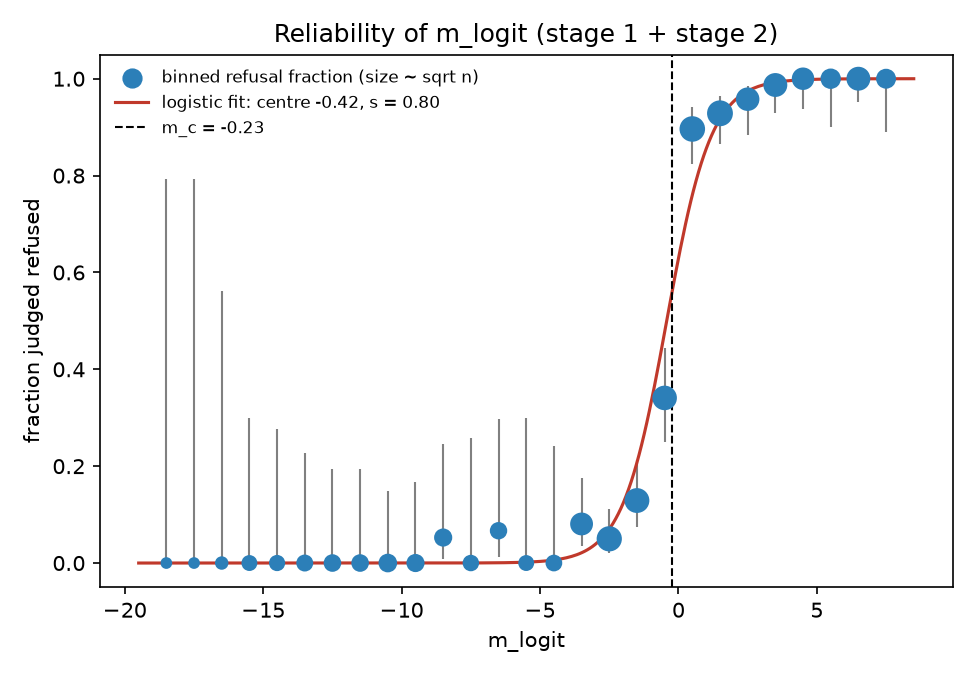
\includegraphics[width=0.6\textwidth]{reliability.png}
\caption{Fraction of completions judged refused, against $m$. The curve is the logistic fit~(\ref{eq:logistic}) and the dashed line is $\mc$.}
\label{fig:reliability}
\end{figure}

Near the threshold the match is looser. Over the 2{,}520 borderline prompts, 89\% of the completions that start with ``I'' are refusals, 8\% are answers and 4\% are unclear. 3\% of the refusals start with another token. For clearly harmful prompts there is no slippage: all 149 completions that start with ``I'' are refusals and no refusal starts otherwise.

One direction controls refusal in this model, as Arditi et al.\ \cite{arditi} reported for other chat models. We call it the \emph{refusal direction}. Later work finds several independent directions that mediate refusal and argues that the single-direction account is incomplete \cite{wollschlager}; nothing below depends on there being only one. Let $r$ be the mean of $h_{13}(t^*)$ over harmful prompts minus its mean over harmless ones, with $t^*$ the fourth template position, and $\hat r=r/\lVert r\rVert$. Removing the component along it, $h\to h-(\hat r\cdot h)\,\hat r$ at every layer and position, takes refusals of 100 harmful prompts from 96 to 0. Adding $r$ to the state at layer 13 at every position takes refusals of 100 harmless prompts from 2 to 100. Removing a random direction instead, isotropic or covariance-matched, leaves 88 to 98\% of the harmful prompts refused.

\subsection{Rewording flips borderline prompts in proportion to their distance from the threshold}
\label{sec:flips}

\begin{table}[ht]
\centering
\caption{Change of $m$ and fraction of flips by kind of rewording, over all pairs of that kind.}
\label{tab:tiers}
\begin{tabular}{lccccc}
\toprule
Kind of rewording & Pairs & Median $|\Dm|$ & Root mean square $\Dm$ & Mean $\Dm$ & Flips \\
\midrule
T0, punctuation & 600 & 0.15 & 0.38 & $+0.06$ & 3\% \\
T1, one or two words & 600 & 0.38 & 1.07 & $+0.11$ & 12\% \\
T2, full rephrasing & 720 & 1.48 & 2.99 & $-0.53$ & 24\% \\
T3, register or context & 480 & 1.05 & 1.99 & $+0.62$ & 21\% \\
\bottomrule
\end{tabular}
\end{table}

\begin{table}[ht]
\centering
\caption{Fraction of flips by the original prompt's distance from the threshold.}
\label{tab:cells}
\begin{tabular}{lcc}
\toprule
Distance $|m-\mc|$ & Flips, answering side & Flips, refusing side \\
\midrule
below 0.9 & 32\% & 25\% \\
0.9 to 1.8 & 27\% & 14\% \\
1.8 to 3.5 & 9\% & 7\% \\
3.5 to 7.1 & 3\% & 3\% \\
\bottomrule
\end{tabular}
\end{table}

That small edits and paraphrases can change a model's answer, and its decision to refuse, is documented \cite{salinas,hughes,anonto}. The tables add rates against a calibrated distance from the threshold. A full rephrasing changes $m$ by a median of 1.5, about twice the width of the transition, and its root mean square change is 3.0 (Table~\ref{tab:tiers}). The root mean square is well above the median for every kind, because a minority of rewordings move $m$ a great deal. For the prompts nearest the threshold, punctuation alone flips about one variant in ten. The flip rate falls with the distance from the threshold on both sides (Table~\ref{tab:cells}). 87 of the 120 prompts have both a refused and an answered completion among their rewordings.

\subsection{Perturbations and rewordings are damped}
\label{sec:damped}

\paragraph{One token at a time.} A perturbation was added to the state at one token at layers 6, 12 and 18 and followed to the last layer, for 43 prompts and about 80 directions each. Figure~\ref{fig:single} shows the one-token relative gain $R$ of~(\ref{eq:gain}). Random directions, differences between real prompts and differences between rewordings all shrink: at the last layer $R$ is 0.07 to 0.20 from layer 6, 0.18 to 0.48 from layer 12, and 0.37 to 0.68 from layer 18. Differences between rewordings follow the covariance-matched random directions in every panel. The refusal direction keeps its size better than random directions from layer 12 on (0.35 to 0.83 against 0.24 to 0.66).

\begin{figure}[ht]
\centering
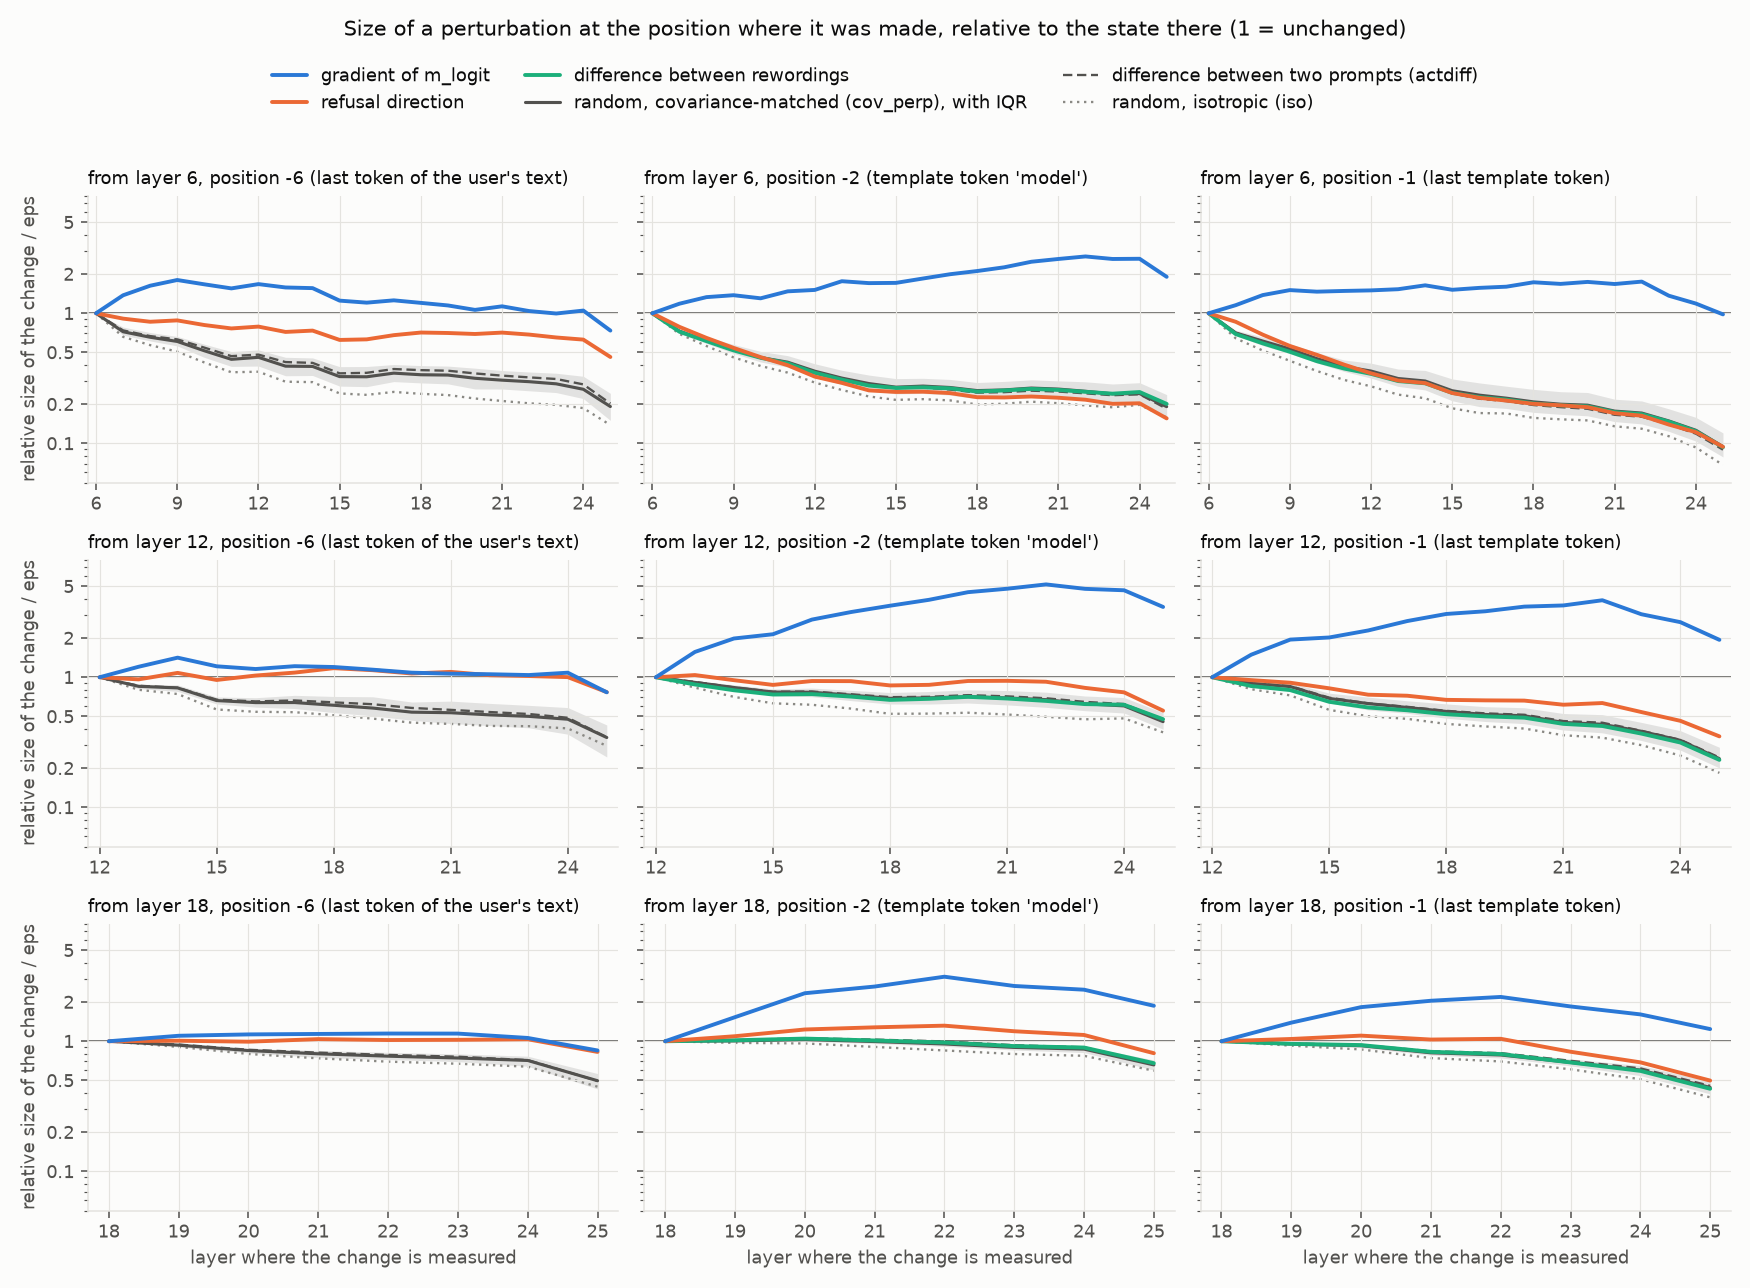
\includegraphics[width=\textwidth]{rgain_same_position.png}
\caption{One-token relative gain $R(\ell\to\ell')$, equation~(\ref{eq:gain}), against the later layer $\ell'$. Each panel is one starting layer and token. Blue: gradient of $m$. Orange: refusal direction. Green: differences between rewordings. Grey: random baselines.}
\label{fig:single}
\end{figure}

\paragraph{All tokens at once.} Perturbations with a total relative size $\varepsilon$ of 1\%, 3\% and 10\% over $S$ were added to the user's tokens at layers 2, 6 and 10 for 16 prompts, with 16 random draws of each kind (Figure~\ref{fig:collective}, right). The all-token gain at the last layer is 0.12 to 0.51 for every kind: one token, an independent direction at every token, and the same direction at every token. At equal total size, the same direction at every token ends within 5\% of the single most sensitive token. Growth on the way is rare and does not last: $R$ exceeded 1 at some intermediate layer in 6\% of 38{,}000 runs, with a largest value of 2.9, and at the last layer in under 1\%.

\paragraph{Real rewordings.} For the 543 one-to-one pairs of Section~\ref{sec:gain}, the relative difference $\varepsilon_\ell(\Delta_\ell;S)$ between the two prompts has a median of 17.5\% at the embeddings and 6.6\% at the last layer. Per pair, the ratio $\varepsilon_{25}/\varepsilon_{-1}$ has a median of 0.42 (Figure~\ref{fig:collective}, left). The ratio rises by 8\% in the first layer and falls after that, and 4 of the 543 pairs end above 1. In absolute size the difference grows 4.7 times while the state grows 12.6 times.

\begin{figure}[ht]
\centering
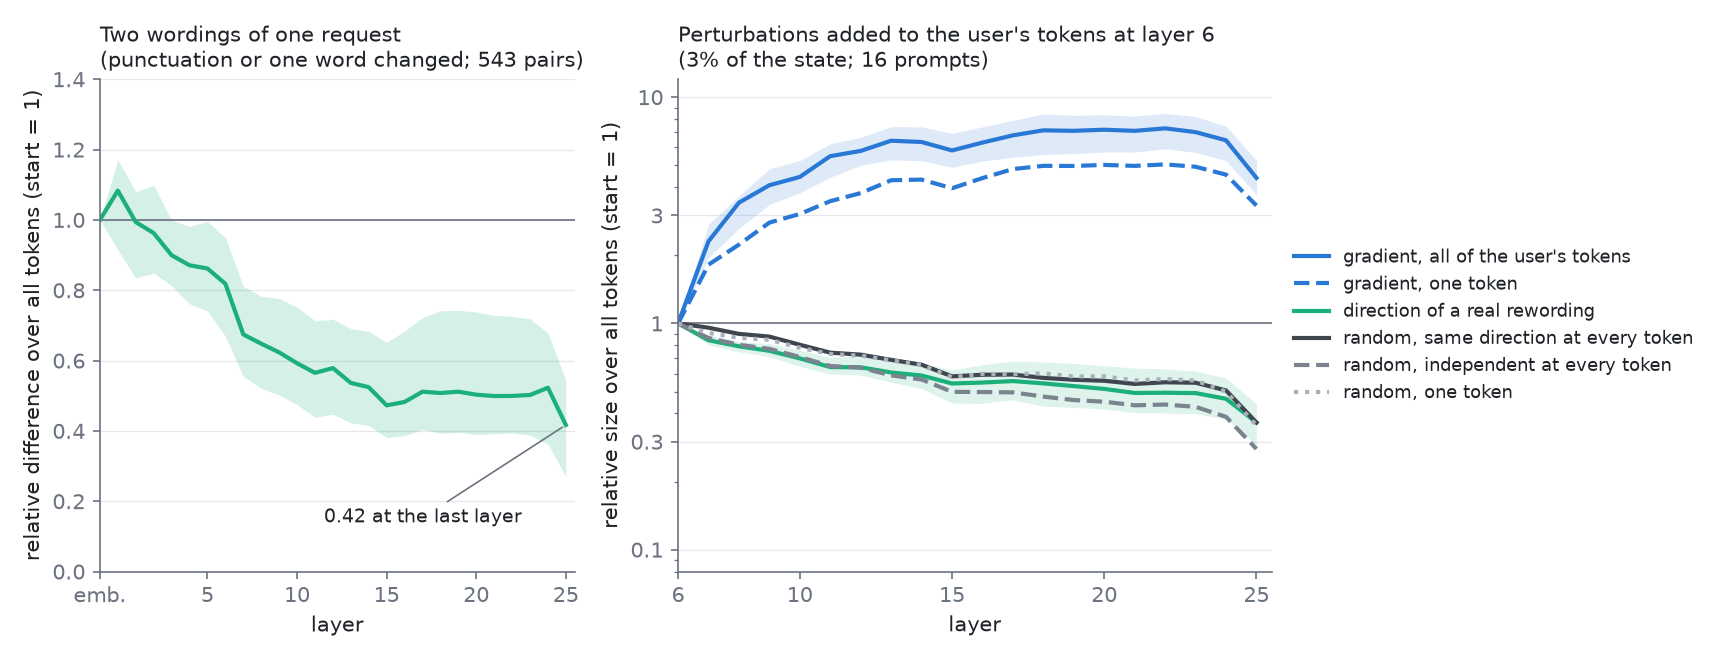
\includegraphics[width=\textwidth]{collective.png}
\caption{Left: $\varepsilon_\ell/\varepsilon_{-1}$ for the difference between two wordings over all tokens. Right: all-token relative gain $R(6\to\ell')$ of perturbations added to the user's tokens at layer 6 with $\varepsilon=0.03$, on a logarithmic scale. Bands hold the middle half of the cases.}
\label{fig:collective}
\end{figure}

The difference also spreads. Its effective number of tokens~(\ref{eq:neff}) is 1 at the embeddings, where only the changed tokens differ, and 3.3 at the last layer, of a median 20 in $S$. Half of the squared difference is still at the changed tokens there.

\subsection{A narrow set of directions is amplified}
\label{sec:amplified}

The gradient of $m$ is the exception in both experiments.

\begin{description}
\item[Growth.] A perturbation with $\varepsilon=0.03$ along the gradient over all the user's tokens reaches an all-token gain of 5 to 7 by layer 22 and ends at 3.3 to 4.5 (Figure~\ref{fig:collective}, blue). Its template gain at the last layer is 8 to 10, and 11 to 21 in the linearized limit.
\item[The most amplified direction.] For 7 prompts the top singular vector of Section~\ref{sec:svd} was computed, with the user's text as the source and with the user's text and the template together. The relative amplification $\mathcal{A}$ of~(\ref{eq:amp}) is 13 to 38, depending on the starting layer and the source. The gradient direction reaches 30 to 95\% of that. A random direction over the same tokens reached 0.7\% of it in the one case checked.
\item[Steepness.] Over all 120 prompts, the steepness $G_\ell$ of~(\ref{eq:G}) has a median of 320 to 490 at every layer from 0 to 15. A perturbation of 0.2\% of the state along the gradient therefore moves $m$ by 0.8, the width of the transition. Prompts in the half nearer the threshold are steeper than the others by 7 to 45\%, depending on the layer.
\item[Saturation of the state.] The response of the state along the gradient is far from linear at the size of real rewordings: at $\varepsilon=0.1$ the template gain is a fifth to a third of its linearized value. The scalar $m$ stays closer to linear (Section~\ref{sec:linrange}).
\item[Many tokens against one.] The gradient over all the user's tokens is 1.3 to 2.2 times as effective as the gradient at the single best token. The top singular value with the user's text as source is 1.7 to 2.3 times that of the most sensitive single token, and its singular vector has $N_{\rm eff}$ of 4 to 6 of a median 14 tokens. The bound~(\ref{eq:bound}) allows a factor $\sqrt N$; the measured factor is 0.45 to 0.7 of $\sqrt N$. The collective modes are therefore sums of a few one-token modes, and there is no separate collective instability.
\end{description}

Real rewordings barely point along these directions. For a small edit the cosine in~(\ref{eq:consistency}) has a median absolute value of 0.003 to 0.004 in layers 0 to 6 and 0.010 at layer 15, against 0.002 to 0.003 for random displacements with the same norm at every token.

These numbers are consistent with each other to within their ranges. In the first six layers a small edit has $\varepsilon$ of 0.13 to 0.17, the steepness is 320 to 490 and the cosine 0.003 to 0.004, so equation~(\ref{eq:consistency}) gives $|\Dm|$ of 0.1 to 0.3. The measured median for these pairs is 0.25.

\subsection{What the gradient direction is}
\label{sec:gradmeaning}

The gradient is the steep direction of Section~\ref{sec:amplified}. At the last layer it has an exact meaning: by~(\ref{eq:m}), $m$ is the logit of ``I'' minus the logarithm of the summed exponentials of all other logits, so the gradient there is the output vector of ``I'' minus the probability-weighted average of the output vectors of the tokens the model would otherwise start with. At earlier layers it is that read-out pulled back through the layers in between, and it depends on the prompt. Three measurements say what it is in practice. They use the gradients $g_\ell(t)$ of the 120 original prompts at the template positions and the states of the 5{,}311 pool prompts. We write $\hat g=g/\lVert g\rVert$, and $r_\ell(t)$ for the difference of means of Section~\ref{sec:scalar} taken at layer $\ell$ and template position $t$, so that $r=r_{13}(t^*)$.

\paragraph{It is mostly one direction, shared by all prompts.} Table~\ref{tab:gradshared} gives the mean cosine $\hat g_f\cdot\hat g_{f'}$ between the gradients of two different prompts, and the share of the squared length of the 120 unit gradients that lies along their first principal direction and along their first ten. Two random directions in 2{,}304 dimensions have a cosine of about 0.014. The gradients are far more alike than that at every layer, and increasingly so with depth. At the last template position the mean cosine is 0.41 at layer 13 and 0.82 at layer 25. Prompts on the same side of the threshold are only slightly more alike than prompts on opposite sides (0.44 against 0.37 at layer 13, last position).

\begin{table}[ht]
\centering
\caption{The gradients of the 120 prompts at the fourth template position $t^*$, by layer: how alike they are, and their cosine with the difference-of-means direction $r_\ell(t^*)$ at the same layer (median over prompts).}
\label{tab:gradshared}
\begin{tabular}{ccccc}
\toprule
Layer & Mean cosine between & Share on first & Share on first ten & Cosine with $r_\ell(t^*)$ \\
 & two prompts & principal direction & principal directions & \\
\midrule
0 & 0.36 & 0.40 & 0.70 & 0.00 \\
6 & 0.35 & 0.39 & 0.67 & 0.03 \\
9 & 0.44 & 0.48 & 0.73 & 0.13 \\
13 & 0.53 & 0.56 & 0.80 & 0.23 \\
15 & 0.59 & 0.62 & 0.84 & 0.25 \\
18 & 0.62 & 0.64 & 0.89 & 0.21 \\
\bottomrule
\end{tabular}
\end{table}

\paragraph{It has a steady component along the refusal direction, and is not the same vector.} The cosine between a prompt's gradient and $r_\ell(t^*)$ is zero up to layer 3 and 0.19 to 0.26 from layer 12 to layer 21 (Table~\ref{tab:gradshared}). From layer 12 on it has the same sign for 97 to 100\% of the prompts.

\paragraph{On real prompts the two read the same coordinate.} Let $\bar g$ be the unit vector along the mean of the $\hat g_f$ at layer 13, position $t^*$; its cosine with $\hat r$ is 0.29. Over the 5{,}311 pool prompts, the projections $\bar g\cdot h$ and $\hat r\cdot h$ of the state have a correlation of 0.96. Each separates harmful from harmless prompts almost perfectly: the ranking probability is 0.999 for $\bar g\cdot h$ and 1.000 for $\hat r\cdot h$, and its median is 0.998 when the gradient of a single prompt is used.

A cosine of 0.3 and a correlation of 0.96 are compatible because the states are strongly anisotropic. The refusal direction is the direction in which prompts differ most: it coincides with the first principal direction of the pool states (cosine 0.98) and holds 28\% of their variance, where an average direction holds $1/2304=0.04\%$. The component of the gradient along $\hat r$ is under a tenth of its squared length, but it multiplies by far the largest variation among real prompts, and so it dominates what the gradient reads from them. The rest of the gradient lies in directions along which real prompts hardly vary.

\paragraph{As a perturbation the gradient is about four times more effective.} To first order, a perturbation of relative size $\varepsilon$ at the single position $(13,t^*)$ along a unit vector $u$ changes $m$ by $\varepsilon\,|g\cdot u|\,\lVert h\rVert$. The median of $|g\cdot u|\,\lVert h\rVert$ over the 120 prompts is 52 along the gradient, 12 along $\hat r$, 1.8 along a covariance-matched random direction and 0.7 along an isotropic one. The refusal direction is therefore 6 to 7 times more effective than a typical direction of real variation, and the gradient 4 times more effective again, by using directions that real prompts do not explore.

\paragraph{Relation to earlier work.} That refusal directions found by gradient-based optimization differ from the difference of means is reported in \cite{wollschlager}, and \cite{park} argue that Euclidean cosines between such directions mean little without an inner product that accounts for the statistics of the states, which is the point of the anisotropy argument above. What is added here is the direct measurement for the local gradient: its cosine with the difference of means, and the correlation of the two projections on real prompts.

\paragraph{A stricter relation that does not hold.} The best linear read-out for separating two Gaussian classes with a common covariance $C$ is the difference of their means multiplied by the inverse covariance, $C^{-1}r$. If the model's read-out were that optimal discriminant, one would find $g\propto C^{-1}r$. This is not what is found: the cosine between $g$ and $C^{-1}r$, with $C$ the covariance of the pool states and a ridge term added for stability, is 0.02 to 0.05, at the level of random directions (0.015).

\paragraph{Reading.} The gradient is a read-out with two parts. One part reads the refusal coordinate, which is where real prompts move. The larger part points where real prompts do not go, which is why a perturbation along the gradient is so effective and so unlike a rewording. A largely shared gradient also fits the negative result of Section~\ref{sec:test}: if the gradient is nearly the same vector for every prompt, a prompt's own gradient says little that distinguishes it from the others. That link has not been tested directly.

\subsection{Linear response describes each flip}
\label{sec:linear}

The difference between two wordings reaches the template positions between layers 6 and 15. The arrival fraction $f_\ell$ of the swap experiment (Section~\ref{sec:swap}) is 0.10 at layer 6, 0.52 at layer 9, 0.76 at layer 12, 0.95 at layer 15 and 1.00 from layer 18 (Figure~\ref{fig:arrival}). Almost nothing the model reads from the user's text after layer 18 affects $m$.

\begin{figure}[ht]
\centering
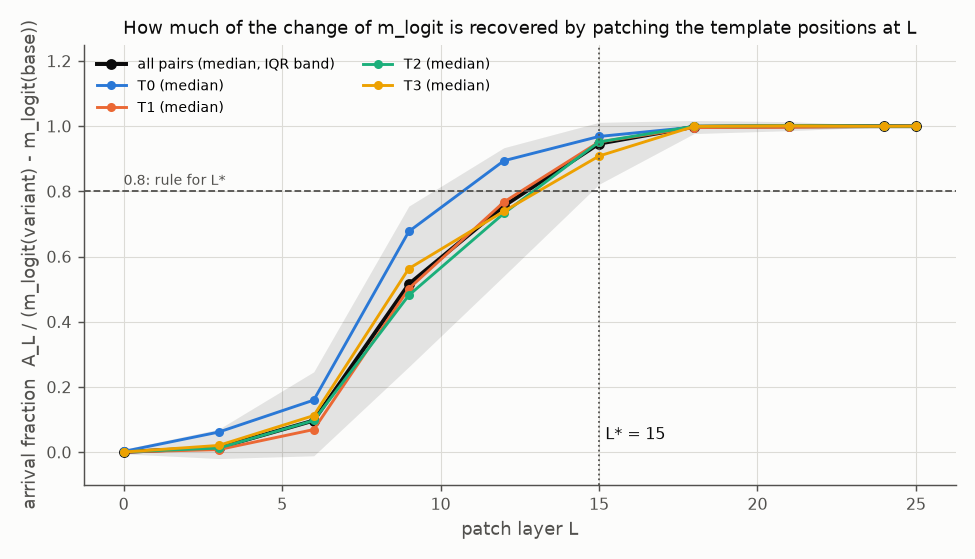
\includegraphics[width=0.7\textwidth]{arrival_curve.png}
\caption{Arrival fraction $f_\ell$, equation~(\ref{eq:arrival}): the fraction of the change in $m$ that is reproduced by swapping the template-position state at layer $\ell$.}
\label{fig:arrival}
\end{figure}

The linear prediction~(\ref{eq:lin}) is the estimate used in attribution patching for the effect of replacing one prompt's activations by another's \cite{kramar}, where it is known to fail when attention saturates or contributions cancel. What is measured here is how well it holds for real rewordings of increasing size. At layer 15, the linear prediction $L_{15}$ of~(\ref{eq:lin}) over the template positions has correlation 0.92 with the actual $\Dm$ and slope 0.99, and the right sign for 99\% of the pairs with $|\Dm|>0.5$ (Figure~\ref{fig:gdelta}). This holds for full rephrasings too; Section~\ref{sec:linrange} measures how far the linear range extends. Changes larger than about 3 fall away from the line.

\begin{figure}[ht]
\centering
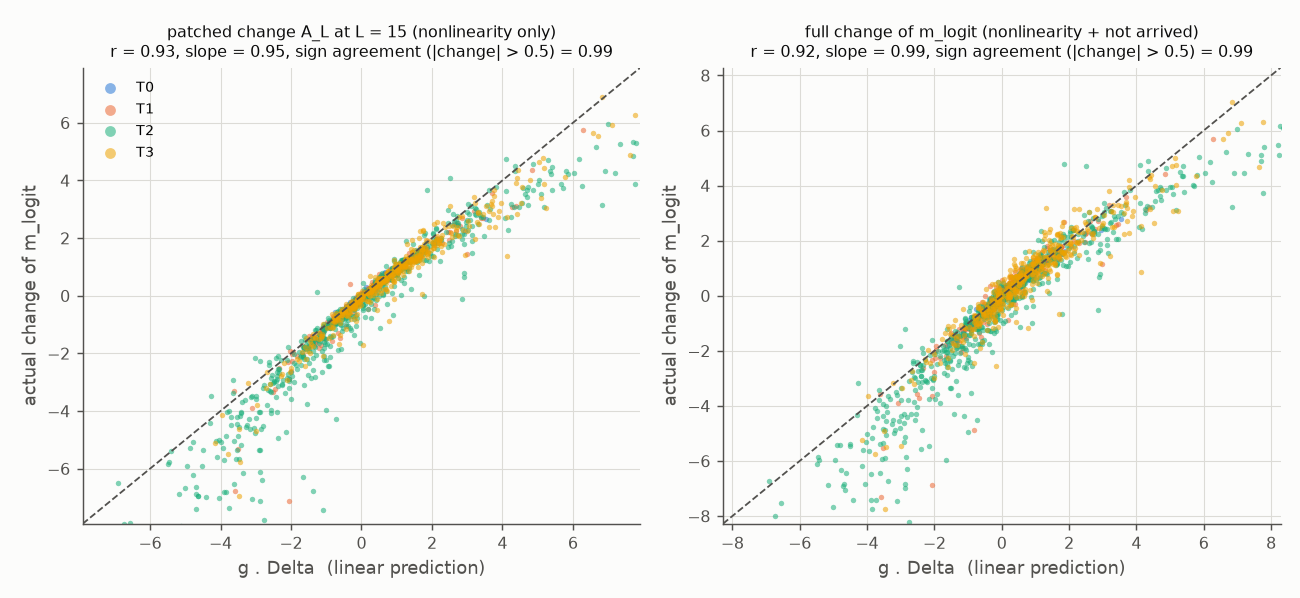
\includegraphics[width=0.8\textwidth]{gdelta_vs_actual.png}
\caption{Linear prediction $L_\ell$ against the actual change $\Dm$; one point per pair of an original and a rewording.}
\label{fig:gdelta}
\end{figure}

For the one-to-one pairs the sum in~(\ref{eq:lin}) can be taken over $S$, the user's text included. It then gives the sign of $\Dm$ from layer 4 (92\% agreement) and its size from layers 12 to 15. It fails at layers 0 to 2, where a swapped token is a change of 80\% of its own state and first order does not apply. The linear description therefore starts only after the edit has been absorbed by the first few layers and cannot be run from the embeddings.

Much of the effect lies along the refusal direction, as Section~\ref{sec:gradmeaning} leads one to expect. Across the 2{,}400 pairs, the change in the projection $\hat r\cdot h_{13}(t^*)$ correlates 0.82 with $\Dm$. This is from a first look during review and was not a planned measurement.

\subsection{How far the linear range extends}
\label{sec:linrange}

The linear prediction works for rephrasings that displace the template state by 15 to 30\%, while the state responds nonlinearly to a 3\% perturbation along the gradient (Section~\ref{sec:amplified}). One explanation would be that the model is close to linear for displacements that stay inside the cloud of real states and nonlinear for those that leave it. We tested this and it is not supported.

Perturbations were made at one template position (layer 13, position $t^*$) for 40 prompts, along 61 directions each, at sizes from 1\% to 100\% of the state and with both signs. The directions are principal directions of the pool states from the largest to the 2{,}048th, the gradient and its parts inside and outside the 32 largest principal directions, the refusal direction, random directions, differences between prompts, and the prompt's own rewordings. The response is the change of the state at the last layer and of $m$. A second site (layer 18, last position) gives the same picture.

\begin{table}[ht]
\centering
\caption{Deviation from linearity by direction, at layer 13, position $t^*$ (medians over 40 prompts). $\kappa$ is the deviation of the last-layer state per unit relative size, the linear range is the size at which the deviation~(\ref{eq:nu}) reaches 0.3, and the last column is the Mahalanobis length of a perturbation of unit relative size. ``Top 32'' means the 32 largest principal directions; the first principal direction is close to the refusal direction.}
\label{tab:linrange}
\begin{tabular}{lccc}
\toprule
Direction & $\kappa$ & Linear range & Mahalanobis length \\
\midrule
Isotropic random & 1.5 & 0.20 & 34 \\
Covariance-matched random & 1.7 & 0.19 & 3.5 \\
Principal directions, 1st to 2{,}048th & 3.0, then 1.4 to 2.1 & 0.19 & 0.1 to 57 \\
Real rewording & 1.8 & 0.18 & 10 \\
Difference between two prompts & 2.1 & 0.15 & 3.2 \\
Refusal direction & 3.0 & 0.12 & 0.3 \\
Gradient, part inside the top 32 & 3.0 & 0.11 & 0.4 \\
Gradient, the rest & 7.5 & 0.043 & 35 \\
Gradient & 7.9 & 0.041 & 33 \\
\bottomrule
\end{tabular}
\end{table}

\begin{description}
\item[Nonlinearity is set by relative size, not by distance from the cloud.] The deviation is proportional to $\varepsilon$ (slope 0.96 in a log-log fit). The criterion fixed before the measurement was that adding the Mahalanobis length to that fit should raise its $R^2$ by at least 0.2, with a coefficient comparable to that of $\varepsilon$. It raises $R^2$ from 0.936 to 0.939. Across the principal directions the Mahalanobis length varies 500-fold while $\kappa$ stays between 1.4 and 2.1 (Table~\ref{tab:linrange}).
\item[A real rewording is no more linear than a random direction.] Its $\kappa$ is that of the random baselines. At its real size the deviation of the last-layer state is 0.06 for punctuation, 0.10 for one word, 0.29 for a rephrasing and 0.24 for a change of register or context, and random directions of the same sizes deviate as much.
\item[$m$ is more linear than the state.] For the same rewordings the deviation $\nu_m$ of $m$ is 0.02, 0.03, 0.11 and 0.14. Over all directions its median is 0.02, 0.08 and 0.23 at $\varepsilon=0.03$, 0.1 and 0.3. Along the gradient at $\varepsilon=0.03$ it is 0.035, where the state deviates by 0.24. This is why the linear prediction of Section~\ref{sec:linear} holds for rephrasings: it is a prediction of $m$, which is within about 15\% of linear at their size.
\item[What does depend on direction.] The linear range of the state is five times shorter along the gradient than along a random direction. The excess comes from the part of the gradient outside the largest principal directions, but an isotropic random direction lies just as far outside the cloud and has one of the smallest $\kappa$ in the table, while the refusal direction lies well inside it and has twice that. In a fit made after seeing these results, and therefore not a test, replacing the Mahalanobis length by the size of the linear response $\lVert D\rVert$ raises $R^2$ from 0.936 to 0.973: directions that the model amplifies more are also more nonlinear.
\end{description}

These are perturbations of a single position with the others held fixed, so they say nothing about nonlinearity that arises when many positions move together.

\subsection{The flip probability is not predicted from the prompt alone}
\label{sec:test}

Table~\ref{tab:headline} gives the scores of the four predictors of Section~\ref{sec:testdef}, with gradients and displacements taken at layer 15.

\begin{table}[ht]
\centering
\caption{The test. $B$ is the Brier score~(\ref{eq:brier}), for which lower is better and a forecast with no skill scores 0.127. The rank correlation is with the observed flip fraction of each prompt. The last two rows use the prompt's own rewordings and are not predictions.}
\label{tab:headline}
\begin{tabular}{llcc}
\toprule
Predictor & $\sigma$ & $B$ & Rank correlation \\
\midrule
Distance to the threshold & (\ref{eq:sigdist}) & 0.1071 & 0.71 \\
Gradient-based prediction & (\ref{eq:siggrad}) & 0.1059 & 0.74 \\
Same formula, own rewordings & (\ref{eq:sigownlin}) & 0.0998 & \\
Own spread (ceiling for this formula) & (\ref{eq:sigown}) & 0.0990 & 0.85 \\
\bottomrule
\end{tabular}
\end{table}

The difference between the first two rows is $-0.0012$ with a 95\% interval of $-0.0035$ to $+0.0012$, so no gain can be claimed. The result is the same at every layer from 9 on. A version that drops the Gaussian assumption, and uses for $P_{\rm flip}$ the fraction of the other prompts' displacements for which $m+g\cdot\Delta$ lies across the threshold, gives $-0.0023$ with interval $-0.0058$ to $+0.0013$.

The third row shows where the prediction fails. Replacing the true changes $\Dm$ by the linear prediction $g\cdot\Delta$ costs almost nothing: rows three and four differ by 0.0008. The loss is in the step from row three to row two, where the prompt's own displacements are replaced by those of other prompts. What does not transfer between prompts is how far rewordings move the state along the gradient. The predicted $\sigma$ of~(\ref{eq:siggrad}) has the right size on average, but its rank correlation with each prompt's actual spread is 0.37, against 0.31 for the length of the gradient alone.

Two further predictors built from the original prompt alone were scored: the length of the gradient, and a ``gross signal'' that adds up the opposing contributions passing through the attention heads of Section~\ref{sec:heads}. Each closes 12 to 15\% of the gap between the first and last rows, and none detectably (gross signal: $-0.0010$, interval $-0.0028$ to $+0.0008$). The gap is 0.0081 and the half-width of the interval about 0.0024, so the test could only have detected a predictor that closed a third or more of the gap. No further predictors will be tried on these 120 prompts, because a later success would be a matter of selection.

\subsection{A few attention heads write the difference}
\label{sec:heads}

The change in $m$ between two wordings was split by layer with~(\ref{eq:source}) and~(\ref{eq:share}), and by attention head with~(\ref{eq:head}).

\begin{itemize}
\item Layers 7, 11 and 13 have shares $w_\ell$ of 0.24, 0.19 and 0.15, together 57\% of the change, and layers 7 to 16 have 91\% (Figure~\ref{fig:layers}).
\item The head shares add up to 0.83, so the first-order split accounts for 83\% of the change. Ten heads carry 63\% of that, and seven carry half (Figure~\ref{fig:heads}). In the notation layer.head they are led by 13.2, 11.1, 7.3, 11.6 and 7.0.
\item These heads read the user's text and not the template tokens.
\item They are largely the same for all four kinds of rewording and across prompts. Computed on two random halves of the 120 prompts, the ranking of heads agrees with rank correlation 0.88, and the ten leading heads carry at least half of the change for 68\% of the prompts.
\item For punctuation and one-word edits, 44\% of what the heads read comes from the edited tokens and 57\% from unchanged later tokens, whose own state shifted because they attended to the edit in earlier layers.
\end{itemize}

\begin{figure}[ht]
\centering
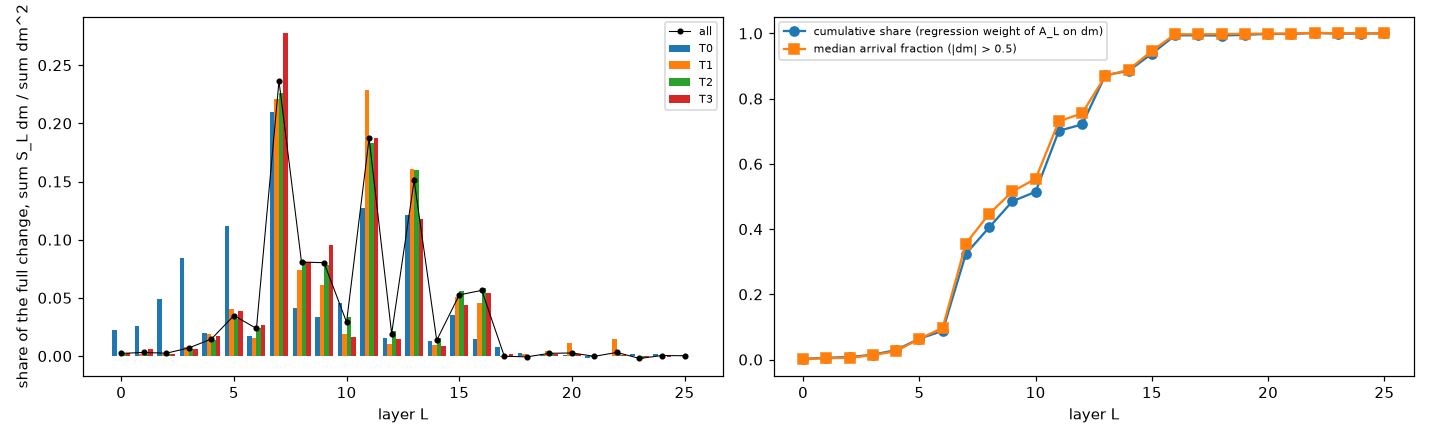
\includegraphics[width=0.75\textwidth]{layers.png}
\caption{Share $w_\ell$ of the change in $m$ written into the template positions at each layer, equation~(\ref{eq:share}).}
\label{fig:layers}
\end{figure}

\begin{figure}[ht]
\centering
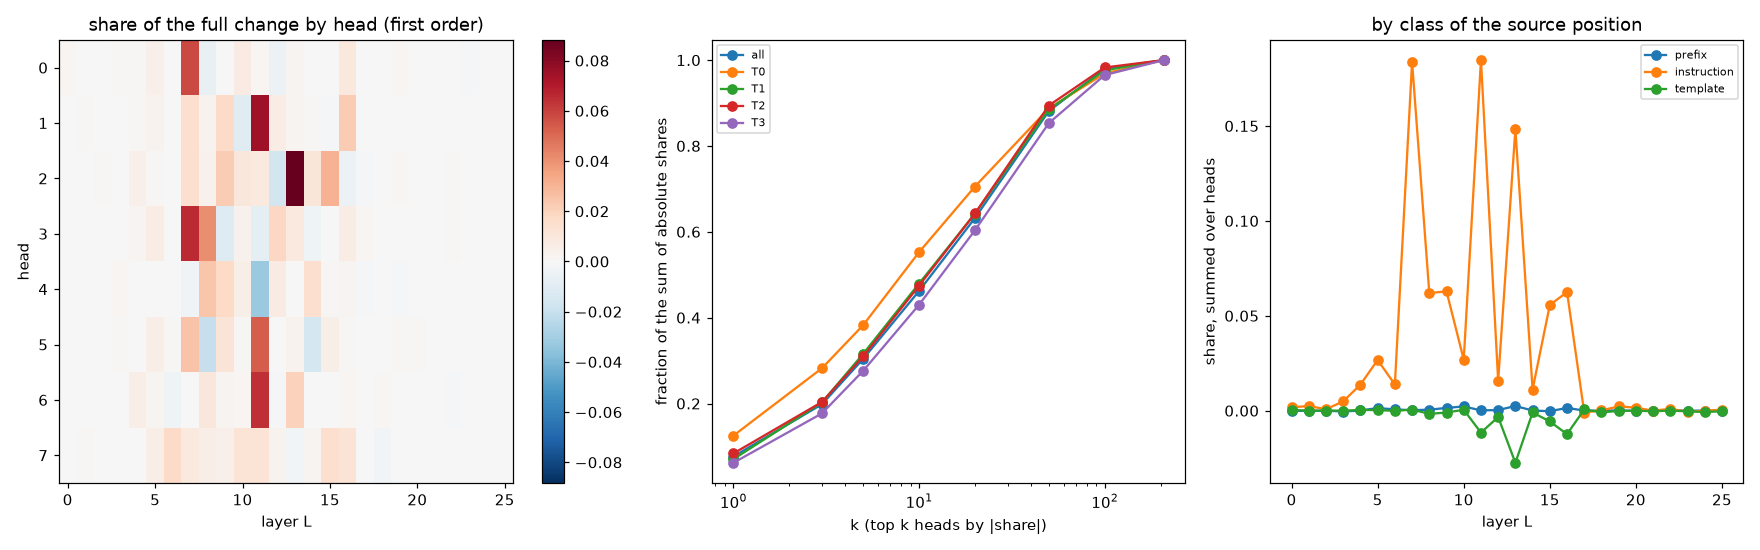
\includegraphics[width=0.75\textwidth]{heads.png}
\caption{Share of the change in $m$ by attention head, from equation~(\ref{eq:head}).}
\label{fig:heads}
\end{figure}

The split by head is an attribution. No head was switched off or swapped, so these heads have not been shown to be necessary or sufficient for a flip.

The mechanism is of a known kind. Attention heads that write to the refusal direction at the last token, and whose attention an adversarial suffix diverts from the instruction, were identified in \cite{arditi}; a suffix attack has been traced to the flow of information into the final template tokens \cite{bentov}; single heads have been scored for their effect on safety by ablation \cite{zhou}; and the template region has been argued to be where safety behaviour is anchored \cite{leong}. Those heads were found by other procedures and mostly in other models, so they cannot be assumed to be the ones found here. What is added is the split, by layer and head, of the difference between two wordings of the same request.

\subsection{A feature-level description was not possible}
\label{sec:features}

Two kinds of published feature dictionary, both trained on the base model and not the chat model, were meant to give a description in terms of interpretable features. Gemma Scope provides autoencoders trained on a chat model only for the larger 9B model \cite{gemmascope}.

\begin{itemize}
\item Sparse autoencoders (Gemma Scope \cite{gemmascope}, 16k features) reproduce 11 to 15\% of the prompt-to-prompt variation at the template positions, against 68 to 76\% on the user's text.
\item With transcoders, 52\% of the influence on the output is unexplained for the chat model, against 26\% for the base model on the same prompts. Nearly all of the gap is at the template positions.
\end{itemize}

The failure is at the positions where the refusal decision is made. For the transcoders the comparison with the base model shows that it comes with the chat fine-tuning. For the autoencoders the same check on the base model was not run, so their failure could also come from template tokens being rare in their training data. Kissane et al.\ \cite{kissane} fine-tuned a base-model autoencoder on chat-model activations for Mistral-7B and recovered the fidelity of a chat-trained one, and Yeo et al.\ \cite{yeo} report continuing the training of Gemma Scope autoencoders on chat data. Neither measured fidelity at the template positions, and no fine-tuning was attempted here.

\section{Interpretation}
\label{sec:interpretation}

This section is a reading of the results, not a further measurement.

For almost every direction in state space the model is contracting in relative terms. A difference between two prompts grows more slowly than the state it sits on, so it matters less and less as depth increases. This holds for random directions, for real rewordings, for one token and for many.

The model is steep along a small number of directions, of which the gradient of $m$ is close to the steepest. Along it, a change of a fraction of a percent decides the outcome. This is what one expects of a system that computes a decision: it has to be sensitive to the quantity it decides on and can afford to be insensitive to the rest. The quantity is largely the same for every prompt, and among real prompts it is the coordinate along the refusal direction (Section~\ref{sec:gradmeaning}).

A rewording is a large perturbation, 13 to 17\% of the state for a one-word edit, that points almost anywhere. In the terms of equation~(\ref{eq:consistency}), the steepness is large, the size is large, and the cosine is under 0.01. Whether the product is enough to cross the threshold depends mostly on how far the original prompt was from the threshold, which is why the distance alone predicts flips about as well as anything computed from the gradient.

This is the picture established for adversarial examples in image classifiers. A model that is close to linear in a high-dimensional input has a few directions along which a small aligned perturbation has a large effect \cite{goodfellow}, while random noise must be larger by a factor of order the square root of the dimension to have the same effect \cite{fawzi}; a real change of the input is neither aligned nor random and mostly misses the steep directions. Stable regions of the residual stream, inside which the output hardly moves, have been described for language models \cite{janiak}. What this study adds is the measurement layer by layer, in relative size, for real rewordings and for refusal.

In the language of the original analogy, there is no instability in the sense of generic perturbations growing with depth. There is one high-gain channel, and wording changes couple to it weakly and in a way that depends on the prompt.

\section{Relation to published work}
\label{sec:related}

A literature check was made after the measurements, by web search (28 searches, 25 works read at least in abstract). Table~\ref{tab:related} gives its verdict for each main claim. No claim was found published in this setting, and most are partly known.

\begin{table}[ht]
\centering
\caption{The main claims against published work. ``Partly known'' means a published result covers the idea or one half of it, but not the measurement or the setting here.}
\label{tab:related}
\small
\begin{tabular}{p{0.40\textwidth}p{0.20\textwidth}p{0.30\textwidth}}
\toprule
Claim & Status & Closest work \\
\midrule
Typical perturbations and real rewordings shrink with depth; only directions near the gradient grow (Sections~\ref{sec:damped}, \ref{sec:amplified}) & partly known & \cite{goodfellow,fawzi,janiak} \\[4pt]
Perturbations over many tokens stay well inside the $\sqrt N$ bound (Section~\ref{sec:amplified}) & apparently new as a measurement & none found \\[4pt]
Linear response for real displacements of 20 to 30\% of the state (Section~\ref{sec:linear}) & partly known & \cite{kramar} \\[4pt]
The linear range of the response, by direction and relative size (Section~\ref{sec:linrange}) & apparently new & \cite{janiak} \\[4pt]
Flip rates by distance from the threshold; prompt-only predictors add nothing (Sections~\ref{sec:flips}, \ref{sec:test}) & partly known & \cite{salinas,hughes,anonto} \\[4pt]
A few heads write the difference into the template positions (Section~\ref{sec:heads}) & partly known & \cite{arditi,bentov,zhou,leong} \\[4pt]
The gradient is a shared direction that reads the refusal coordinate (Section~\ref{sec:gradmeaning}) & partly known & \cite{wollschlager,park} \\[4pt]
Base-model dictionaries lose fidelity at the template positions (Section~\ref{sec:features}) & partly known & \cite{gemmascope,kissane,minder,yeo} \\
\bottomrule
\end{tabular}
\end{table}

The overall picture, the kind of mechanism and the geometry of the two directions are therefore in print in some form. What was not found is the set of measurements: relative size against depth for real rewordings; perturbations over many tokens against the $\sqrt N$ bound; the linear range by direction; flip rates against a calibrated distance, with the negative result for predictors built from the prompt alone; the split by layer and head of the difference between two wordings; and the measured cosine and correlation of the gradient and the difference of means.

``Not found'' is a weak statement here. The search used a web search engine and no citation index, and it was thinnest for the claim about many tokens. The works on dictionaries include crosscoders trained jointly on this model and its base \cite{minder} and Gemma Scope autoencoders trained further on chat data \cite{yeo}; whether any of them does better at the template positions has not been checked.

\section{Limitations}
\label{sec:limitations}

\begin{enumerate}
\item \textbf{One model, one behaviour.} All results are for Gemma-2-2b-it and for refusal read off the first output token. Nothing here shows that larger models or other behaviours are the same.
\item \textbf{The outcome is not binary near the threshold.} About one completion in six there is neither a clear refusal nor a clear answer within 48 tokens. The flip~(\ref{eq:flip}) is therefore a crossing of $\mc$ by $m$, not a change in what the model writes. The two do not always coincide: among the 2{,}010 pairs with a clear label for both prompts, 190 flip on both definitions, 78 cross $\mc$ without a change of label, and 85 change label without crossing $\mc$.
\item \textbf{The judge is rule-based and lightly audited.} Its only audits were done by the session that wrote the rules: on 150 rewording completions the agreement was 0.81, and 0.99 where both gave a clear label.
\item \textbf{The 120 prompts are not a clean sample.} 40 candidates were dropped and replaced because the language models writing the rewordings would not reword them, mostly on the refusing side. Of about 1{,}800 written rewordings, 100 were read against their originals.
\item \textbf{The prompts span a wide range of distances from the threshold.} This makes the distance a strong predictor here and leaves little room to improve on it. Among prompts that are all near the threshold, a prediction of the spread would matter more, and that has not been tested.
\item \textbf{The Gaussian model is approximate.} The shifts are not centred for the larger rewordings and their pooled distribution has heavy tails (Section~\ref{sec:testdef}). The version of the test without the Gaussian assumption gives the same conclusion.
\item \textbf{Reduced samples.} The one-token sweep covered 43 of 60 planned prompts. The many-token perturbations used 16 prompts where 30 or more were planned, and the most amplified directions 7 where 10 were planned. The contrasts reported from them are a factor of 10 and hold for every prompt, but the ratios of many-token to one-token amplification are loose.
\item \textbf{The heads are attributed, not tested.} See Section~\ref{sec:heads}.
\item \textbf{How the work was done.} The code and analyses were written by AI sessions, one work package each. A separate planning session reviewed each package and recomputed its main numbers with independent code, and for the last package repeated three measurements on the model through a different code path. The analysis of Section~\ref{sec:gradmeaning} was done by the planning session itself and has not been recomputed independently. No one else has audited the code.
\item \textbf{The literature comparison is a web search.} Section~\ref{sec:related} rests on 28 searches without a citation index. Several of the cited works were read only in abstract, and no number is quoted from them.
\end{enumerate}

\section{Open questions}
\label{sec:open}

\begin{itemize}
\item \textbf{Are the heads of Section~\ref{sec:heads} causal?} Swapping only those heads' reading between two wordings, against random sets of heads of the same number, would show it.
\item \textbf{What sets the cosine in equation~(\ref{eq:consistency})?} The flip is decided by under 1\% of the displacement, and three attempts to predict its typical size from the original prompt have failed. Section~\ref{sec:gradmeaning} suggests looking at how far a rewording moves the state along the refusal direction, a single coordinate shared by all prompts.
\item \textbf{What does the gradient read at the user's tokens?} Section~\ref{sec:gradmeaning} covers the template positions only. In the early layers most of the sensitivity is at the user's tokens, where the published feature dictionaries still work.
\item \textbf{A feature-level description.} It needs dictionaries that work at the template positions of the chat model.
\item \textbf{Does this hold for larger models and other behaviours?}
\end{itemize}

\begin{thebibliography}{99}

\bibitem{arditi}
A.~Arditi, O.~Obeso, A.~Syed, D.~Paleka, N.~Panickssery, W.~Gurnee and N.~Nanda,
``Refusal in Language Models Is Mediated by a Single Direction,''
arXiv:2406.11717 (2024).

\bibitem{gemmascope}
T.~Lieberum, S.~Rajamanoharan, A.~Conmy, L.~Smith, N.~Sonnerat, V.~Varma, J.~Kram\'ar, A.~Dragan, R.~Shah and N.~Nanda,
``Gemma Scope: Open Sparse Autoencoders Everywhere All At Once on Gemma 2,''
arXiv:2408.05147 (2024).

\bibitem{kissane}
C.~Kissane, R.~Krzyzanowski, A.~Conmy and N.~Nanda,
``SAEs (usually) Transfer Between Base and Chat Models,''
AI Alignment Forum (2024).

\bibitem{yeo}
W.~J.~Yeo, N.~Prakash, C.~Neo, R.~K.-W.~Lee, E.~Cambria and R.~Satapathy,
``Understanding Refusal in Language Models with Sparse Autoencoders,''
arXiv:2505.23556 (2025).

\bibitem{goodfellow}
I.~J.~Goodfellow, J.~Shlens and C.~Szegedy,
``Explaining and Harnessing Adversarial Examples,''
arXiv:1412.6572 (2014).

\bibitem{fawzi}
A.~Fawzi, S.-M.~Moosavi-Dezfooli and P.~Frossard,
``Robustness of classifiers: from adversarial to random noise,''
arXiv:1608.08967 (2016).

\bibitem{janiak}
J.~Janiak, J.~Karwowski, C.~S.~Mangat, G.~Giglemiani, N.~Petrova and S.~Heimersheim,
``Characterizing stable regions in the residual stream of LLMs,''
arXiv:2409.17113 (2024).

\bibitem{kramar}
J.~Kram\'ar, T.~Lieberum, R.~Shah and N.~Nanda,
``AtP*: An efficient and scalable method for localizing LLM behaviour to components,''
arXiv:2403.00745 (2024).

\bibitem{park}
K.~Park, Y.~J.~Choe and V.~Veitch,
``The Linear Representation Hypothesis and the Geometry of Large Language Models,''
arXiv:2311.03658 (2023).

\bibitem{wollschlager}
T.~Wollschl\"ager, J.~Elstner, S.~Geisler, V.~Cohen-Addad, S.~G\"unnemann and J.~Gasteiger,
``The Geometry of Refusal in Large Language Models: Concept Cones and Representational Independence,''
arXiv:2502.17420 (2025).

\bibitem{bentov}
M.~Ben-Tov, M.~Geva and M.~Sharif,
``Universal Jailbreak Suffixes Are Strong Attention Hijackers,''
arXiv:2506.12880 (2025).

\bibitem{zhou}
Z.~Zhou et al.,
``On the Role of Attention Heads in Large Language Model Safety,''
arXiv:2410.13708 (2024).

\bibitem{leong}
C.~T.~Leong, Q.~Yin, J.~Wang and W.~Li,
``Why Safeguarded Ships Run Aground? Aligned Large Language Models' Safety Mechanisms Tend to Be Anchored in The Template Region,''
arXiv:2502.13946 (2025).

\bibitem{salinas}
A.~Salinas and F.~Morstatter,
``The Butterfly Effect of Altering Prompts: How Small Changes and Jailbreaks Affect Large Language Model Performance,''
arXiv:2401.03729 (2024).

\bibitem{hughes}
J.~Hughes et al.,
``Best-of-N Jailbreaking,''
arXiv:2412.03556 (2024).

\bibitem{anonto}
R.~A.~Anonto, M.~L.~A.~Nahiyan and M.~T.~Hassan,
``How Semantically Stable Are LLM Refusals? Measuring Confusion in Local Safety Boundaries,''
arXiv:2512.01037 (2025).

\bibitem{minder}
J.~Minder, C.~Dumas, C.~Juang, B.~Chugtai and N.~Nanda,
``Overcoming Sparsity Artifacts in Crosscoders to Interpret Chat-Tuning,''
arXiv:2504.02922 (2025).

\bibitem{advbench}
A.~Zou, Z.~Wang, N.~Carlini, M.~Nasr, J.~Z.~Kolter and M.~Fredrikson,
``Universal and Transferable Adversarial Attacks on Aligned Language Models,''
arXiv:2307.15043 (2023).

\bibitem{harmbench}
M.~Mazeika et al.,
``HarmBench: A Standardized Evaluation Framework for Automated Red Teaming and Robust Refusal,''
arXiv:2402.04249 (2024).

\bibitem{jbb}
P.~Chao et al.,
``JailbreakBench: An Open Robustness Benchmark for Jailbreaking Large Language Models,''
arXiv:2404.01318 (2024).

\bibitem{orbench}
J.~Cui, W.-L.~Chiang, I.~Stoica and C.-J.~Hsieh,
``OR-Bench: An Over-Refusal Benchmark for Large Language Models,''
arXiv:2405.20947 (2024).

\bibitem{xstest}
P.~R\"ottger, H.~R.~Kirk, B.~Vidgen, G.~Attanasio, F.~Bianchi and D.~Hovy,
``XSTest: A Test Suite for Identifying Exaggerated Safety Behaviours in Large Language Models,''
arXiv:2308.01263 (2023).

\bibitem{alpaca}
R.~Taori et al.,
``Stanford Alpaca: An Instruction-following LLaMA Model,''
\url{https://github.com/tatsu-lab/stanford_alpaca} (2023).

\end{thebibliography}

\end{document}
